
The Calibration Consortium was formed in November 2018 as a joint single and dual phase consortium, with a Consortium Leader and a Technical Leader. The organization of the consortium is shown in Figure~\ref{fig:orgchart}. The calibration consortium board currently comprises institutional representatives from 11 institutes as shown in Table~\ref{tab:gen-calib-org}. The consortium leader is the spokesperson for the consortium and responsible for the overall scientific program and management of the group. The technical leader of the consortium is responsible for managing the project for the group. 

The consortium's initial mandate is the design and prototyping of a laser calibration system, a neutron generator, and a possible radioactive source system and therefore the Consortium is organized in three working groups, each dedicated to each of these systems. Each group has a designated working group leader.
The \dword{tdr} editors are responsible for the overall editing and delivery of the \dword{tdr} document.

\begin{figure}[tbp]
\centering
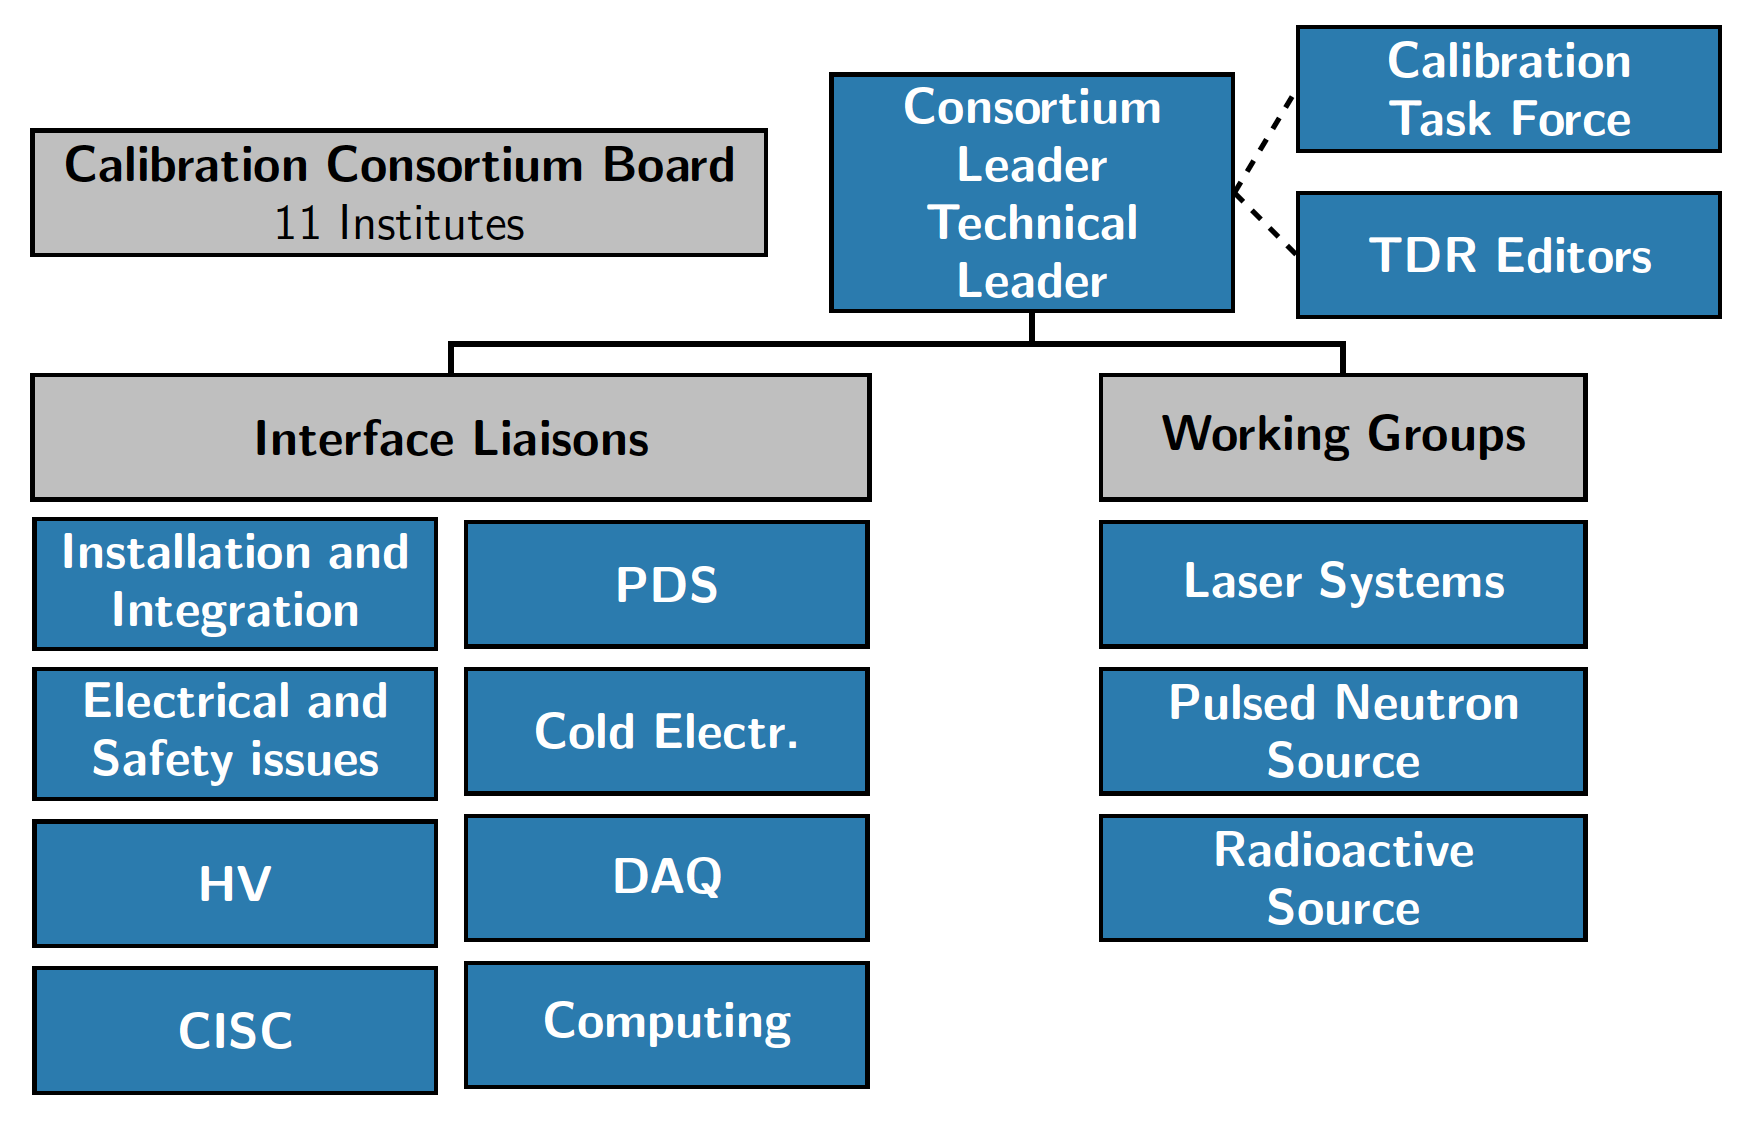
\includegraphics[height=3.0in]{graphics/orgchart.png}
\caption{Organizational chart for the Calibration Consortium.}
\label{fig:orgchart}
\end{figure}

\begin{dunetable}
[Calibration Consortium Institutions]
{lc}
{tab:gen-calib-org}
{Current Calibration Consortium Board institutional members and countries}
Member Institute     &  Country       \\
LIP & Portugal \\ \colhline
University of Bern (Bern) & Switzerland \\ \colhline
University of Tennessee, Knoxville (UTK) & USA \\ \colhline
Michigan State University (MSU) & USA \\ \colhline
Colorado State University (CSU) & USA \\ \colhline
University of Iowa & USA \\ \colhline
University of Hawaii (Hawaii) & USA \\ \colhline
University of Pittsburgh (Pitt) & USA \\ \colhline
Boston University (BU) & USA \\ \colhline
University of California, Davis (UC Davis)& USA \\ \colhline
South Dakota School of Mines and Technology (SDSMT) & USA \\ \colhline
\end{dunetable}

In addition, as shown in Fig.~\ref{fig:orgchart}, there are several liaison roles that are currently being established 
%\todo{These are being established after we have had initial interfaces and critical issues clarified} 
to facilitate the connection with other groups and activities:
\begin{itemize}
    \item Detector Integration and Installation
    \item Electrical and Safety Issues
    \item DAQ
    \item Computing
    \item Cryogenic Instrumentation and Slow Controls
    \item Cold Electronics
    \item High Voltage
    \item Photon Detection System
\end{itemize}

%\fixme{KM adjusted above from "planned" to state will exist by Summer 2019}

Currently, members from new institutes are added to the consortium based on consensus from the consortium board members following an expression of interest petition from the new institute.